%第3章


\section{要求定義}


商品識別システムがどのように機能すべきかという振る舞いと,その外部環境を表すためにユースケース図を作成した.以下に最初に作成した図\ref{usecase1}を載せる.

\begin{figure}[htbp]
\centering
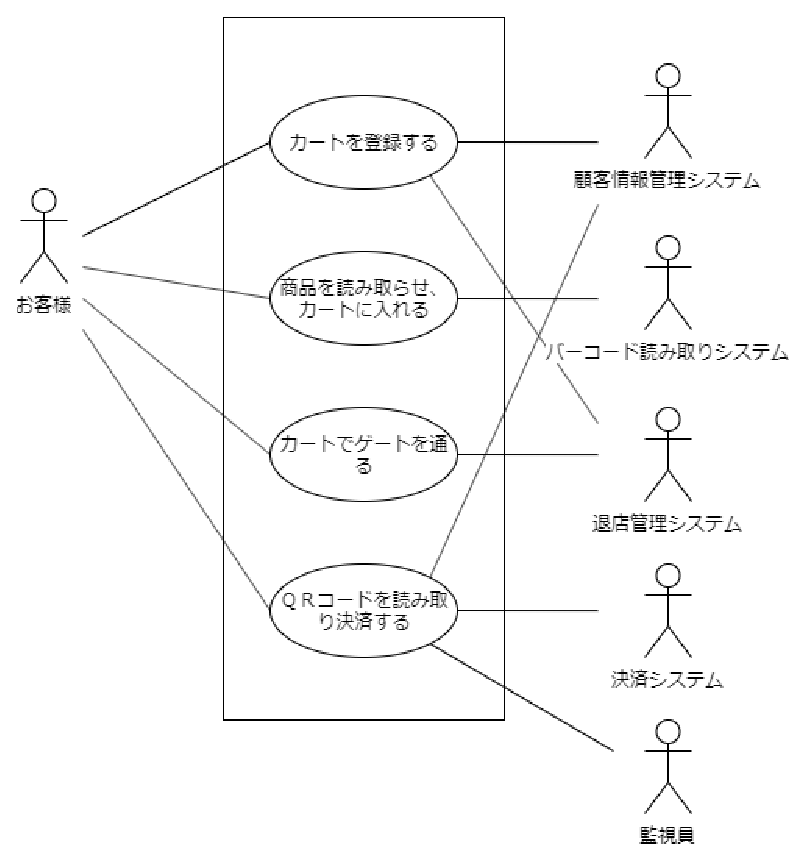
\includegraphics[width = 9cm]{./picture/usecase1.eps}
\caption{ユースケース図(1)}
\label{usecase1}
\end{figure}


図\ref{usecase1}においてユースケースとしてはカゴの登録,商品をカゴに入れる,カゴを持ってゲートを通る,QRコードを読み取り決済するの4つとした.カゴ情報と顧客情報の管理をカゴの登録とカゴでゲートを通るの2つのユースケースで行おうと設計したが,簡単に決済まで行えるという前提から,ユースケースの数が少ないほうが手順が減り簡単という評価軸により適すると考え,ユースケースを見直し,全体のユースケース数を削減した.

%退店管理がどうなってたか思い出せないため,usecase2の図はお蔵入り予定
%\begin{figure}[htbp]
%\centering
%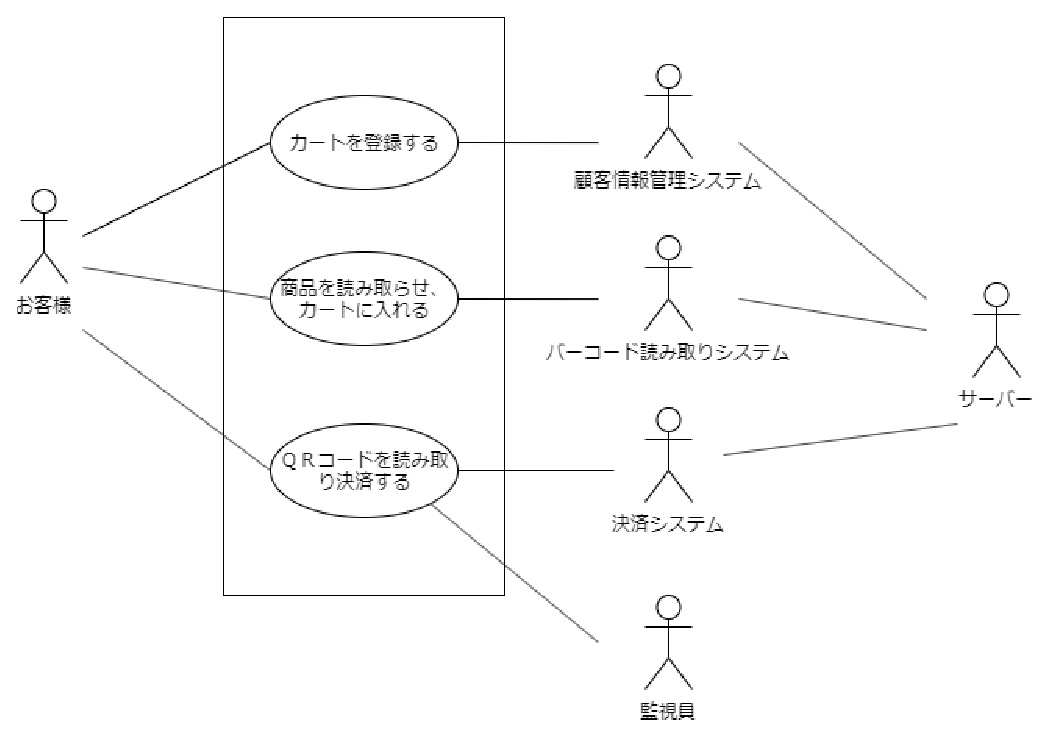
\includegraphics[width = 11cm]{./picture/usecase2.eps}
%\caption{ユースケース図(2)}
%\label{usecase2}
%\end{figure}

ユースケースを見直しユースケースの数を減らしたユースケース図は図\ref{usecase3}に示す.

\begin{figure}[htbp]
\centering
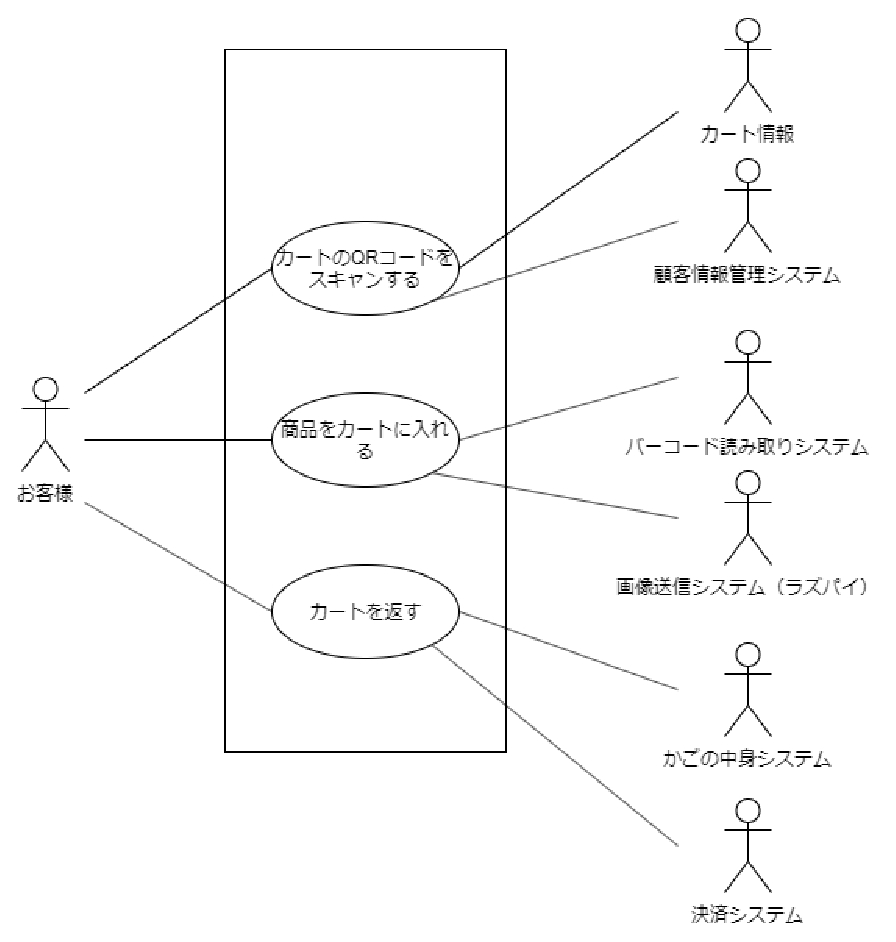
\includegraphics[height = 9cm,width = 9cm]{./picture/usecase3.eps}
\caption{ユースケース図(2)}
\label{usecase3}
\end{figure}


図\ref{usecase3}では,QRコードを読み取り決済していた部分を,カゴの返却時カゴの情報と顧客情報と結び付け,自動的に決済を行う仕様としたためユースケースが3つとなりより簡素化された.登録・買い物・決済の3つのユースケースである.

また,買い物の段階で商品の画像を送信することを考慮した際,カゴに取り付けることのできる小型サイズであり低価格かつ低消費電力のシングルボードコンピュータを用いることとした.シングルボードコンピュータとしては,複数のタスクを動かすことができ,ネットワーク接続に長けたRaspberry Piを選定した.

ここで,問題となったのは登録として,カゴ情報と顧客情報を結びつけたり,解除したりする方法である.QRコードを用いる案と,ICタグを用いる案の2つの案について検討すべく,それぞれの案についてシナリオとユースケース図を作成し,後に優先度の高い範囲を部分を切り出した.


QRコードを用いた場合の商品識別システムのシナリオは下記の表\ref{sina_qr}のとおりである.


\begin{table}[htb]
\begin{center}
\caption{QRコードを用いたシステムのシナリオ}
\begin{tabular}{|l|c|} \hline
 & シナリオ \\ \hline \hline
登録 & カゴのQRコードを顧客が読み取る \\
買い物 & 商品を置く→バーコード認識→商品DB追加・削除→結果通知 \\
決済 & カゴのQRコードをゲートが読み取る→決済を行う \\ \hline
\end{tabular}
\label{sina_qr}
\end{center}
\end{table}

また,QRコードを用いた商品識別システムのユースケース図を図\ref{usecase_qr}に示す.

\begin{figure}[htbp]
\centering
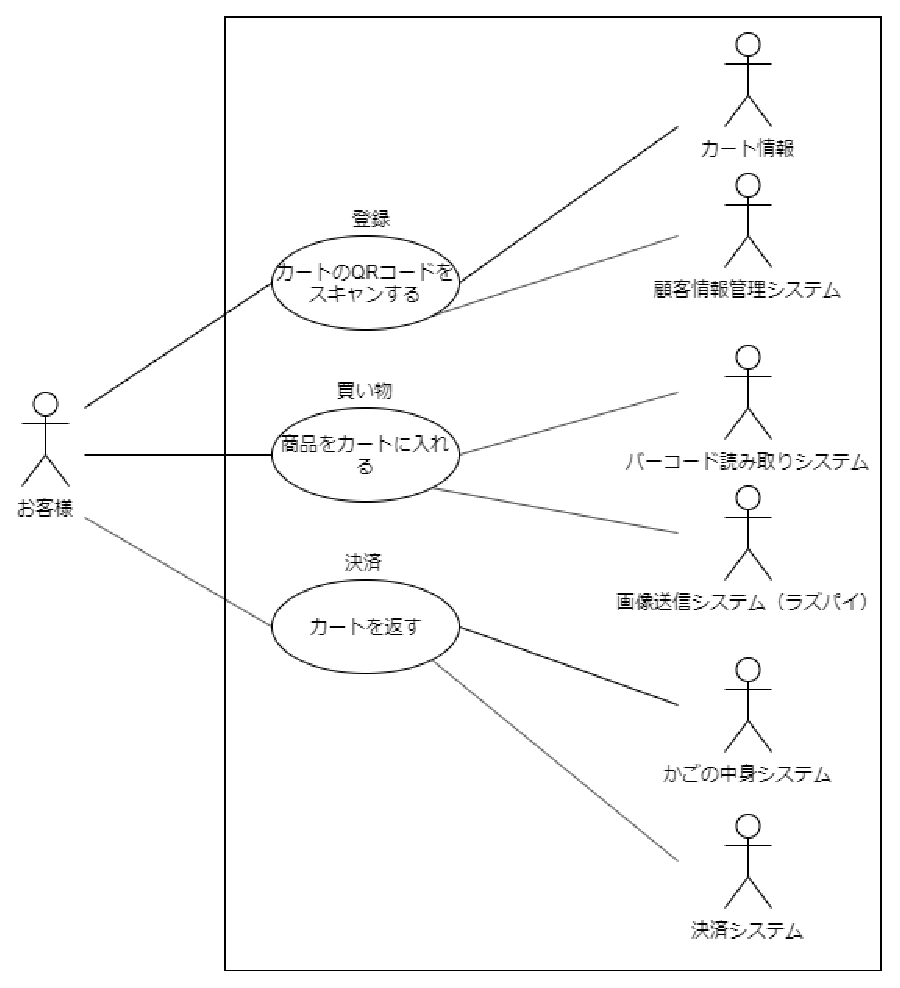
\includegraphics[height = 9cm,width = 9cm]{./picture/usecase_qr.eps}
\caption{QRコードを用いたシステムのユースケース図}
\label{usecase_qr}
\end{figure}

図\ref{usecase_qr}においては,まずカゴにQRコードを印刷したものを貼りつける.QRコードには固有のカゴ情報が含まれており,読み取るとWebページへ遷移し顧客情報を入力する流れとなる.QRコードを入店時顧客が携帯電話等で読み取り,カゴ情報を顧客情報を結びつける.退店時は出口ゲートに設置したWebカメラでカゴのQRコードを読み取り,カゴ情報と顧客情報を管理する.


次に,ICタグを用いた場合の商品識別システムのシナリオを下記の表\ref{sina_ic}へ,ICタグを用いた商品識別システムのユースケース図を図\ref{usecase_ic}に示す.


\begin{table}[htb]
\begin{center}
\caption{ICタグを用いたシステムのシナリオ}
\begin{tabular}{|l|c|} \hline
 & シナリオ \\ \hline \hline
登録 & カゴのICタグをゲートが読み取る \\
買い物 & 商品を置く→バーコード認識→商品DB追加・削除→結果通知 \\
決済 & カゴのICタグをゲートが読み取る→決済を行う \\ \hline
\end{tabular}
\label{sina_ic}
\end{center}
\end{table}


\begin{figure}[htbp]
\centering
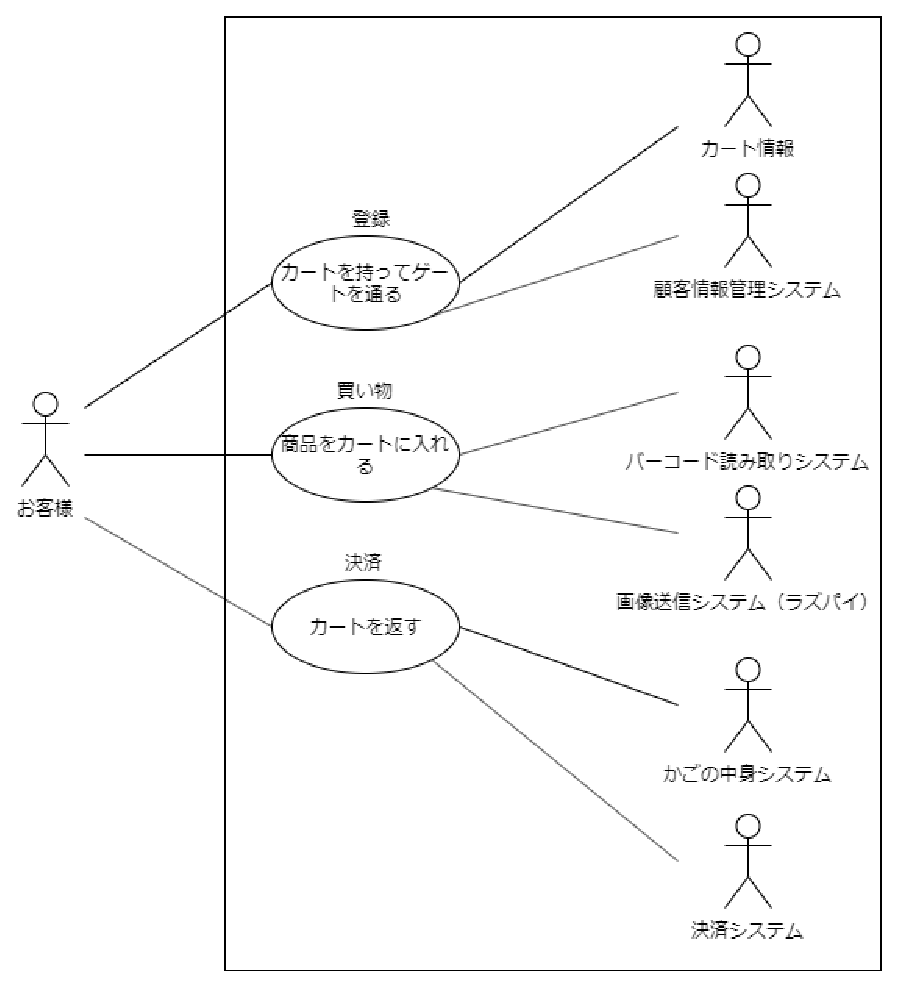
\includegraphics[height = 9cm,width = 9cm]{./picture/usecase_ic.eps}
\caption{ICタグを用いたシステムのユースケース図}
\label{usecase_ic}
\end{figure}

図\ref{usecase_ic}においては,カートもしくはカゴにICタグを取り付け,入退店時にリーダーを設置したゲートを通ることで,カゴ情報と顧客情報を管理する.

%以下は3-2もしくは3-3で評価しようかな(下記の記述移動可能性)

それぞれの入退店時の案について基本の評価軸を用い,下記の表\ref{test}で評価した.


\begin{table}[htb]
\begin{center}
\caption{評価表}
\begin{tabular}{|l||c|c|} \hline
 & QRコード & ICタグ \\ \hline \hline
従来のセルフレジよりコストは抑えられるか & 〇 & × \\
既存の中小店でも導入が容易か & 〇 & △ \\
従来のセルフレジより簡単な動作で決済まで行えるか & × & 〇 \\ \hline
\end{tabular}
\label{test}
  \end{center}
\end{table}


%具体的なカメラの台数やICタグの価格等を下記へ
評価した結果,よりQRコードを用いる案のほうがコストの面で優れている.しかしながら,簡単に決済まで行えるかという基準においては,携帯電話のカメラを起動して読み込む動作を顧客が行わなければならない点からQRコードを用いる案はあまり優れていないといえる.要求分析の段階ではどちらの案がよいかはかりかねたため,基本設計・詳細設計までそれぞれの案について設計した.

また,最終的に本研究で実装対象とした優先度の高い項目部分においてのシナリオ,ユースケース図は下記の図\ref{use}と表\ref{sina}のとおりである.


\begin{figure}[htbp]
\centering
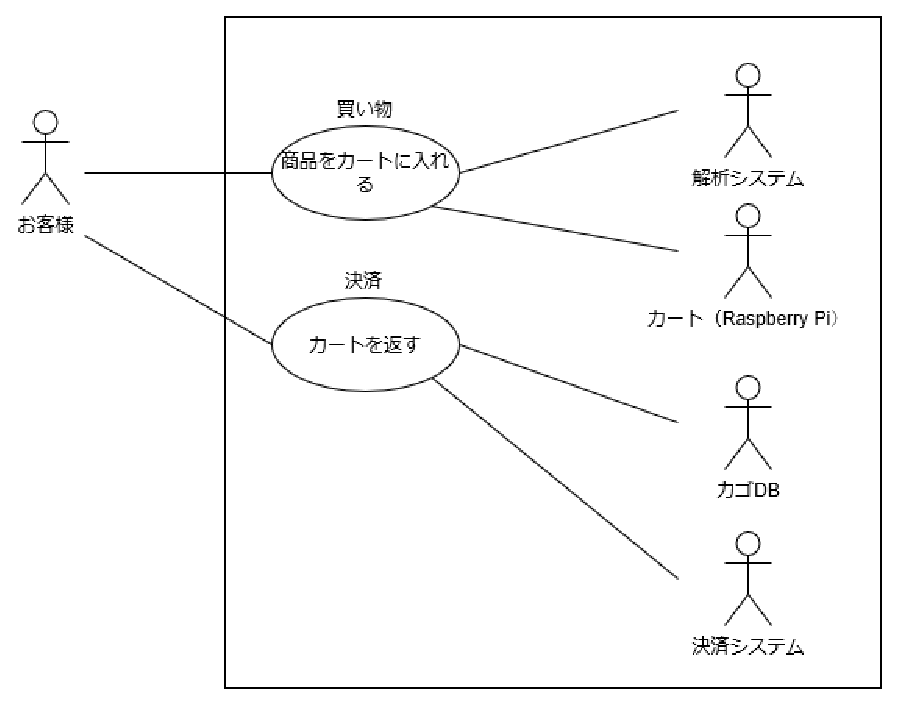
\includegraphics[width = 9cm]{./picture/usecase_saishu.eps}
\caption{高優先度のシステムのユースケース図}
\label{use}
\end{figure}

\begin{table}[htbp]
\begin{center}
\caption{高優先度のシステムのシナリオ}
\begin{tabular}{|l|c|} \hline
 & シナリオ \\ \hline \hline
買い物 & 商品を置く→バーコード認識→商品DB追加・削除→結果通知 \\
決済 & 決済を行う \\ \hline
\end{tabular}
\label{sina}
\end{center}
\end{table}




\newpage